%  LaTeX support: latex@mdpi.com 
%  In case you need support, please attach all files that are necessary for compiling as well as the log file, and specify the details of your LaTeX setup (which operating system and LaTeX version / tools you are using).

% You need to save the "mdpi.cls" and "mdpi.bst" files into the same folder as this template file.

%=================================================================
\documentclass[bioengineering,article,submit,moreauthors,pdftex,10pt,a4paper]{mdpi} 
%
%--------------------
% Class Options:
%--------------------
% journal
%----------
% Choose between the following MDPI journals:
% actuators, admsci, aerospace, agriculture, agronomy, algorithms, animals, antibiotics, antibodies, antioxidants, applsci, arts, atmosphere, atoms, axioms, batteries, bdcc, behavsci, beverages, bioengineering, biology, biomedicines, biomimetics, biomolecules, biosensors, brainsci, buildings, carbon, cancers, catalysts, cells, challenges, chemengineering, chemosensors, children, chromatography, climate, coatings, computation, computers, condensedmatter, cosmetics, cryptography, crystals, data, dentistry, designs, diagnostics, diseases, diversity, econometrics, economies, education, electronics, energies, entropy, environments, epigenomes, fermentation, fibers, fishes, fluids, foods, forests, fractalfract, futureinternet, galaxies, games, gastrointestdisord, gels, genealogy, genes, geosciences, geriatrics, healthcare, horticulturae, humanities, hydrology, informatics, information, infrastructures, inorganics, insects, instruments, ijerph, ijfs, ijms, ijgi, ijtpp, inventions, jcdd, jcm, jcs, jdb, jfb, jfmk, jimaging, jof, jintelligence, jlpea, jmse, jpm, jrfm, jsan, land, languages, laws, life, literature, logistics, lubricants, machines, magnetochemistry, marinedrugs, materials, mathematics, mca, mti, medsci, medicines, membranes, metabolites, metals, microarrays, micromachines, microorganisms, minerals, molbank, molecules, mps, nanomaterials, ncrna, neonatalscreening, nitrogen, nutrients, ohbm, particles, pathogens, pharmaceuticals, pharmaceutics, pharmacy, philosophies, photonics, plants, polymers, proceedings, processes, proteomes, publications, quaternary, qubs, recycling, religions, remotesensing, resources, risks, robotics, safety, scipharm, sensors, separations, sexes, sinusitis, socsci, societies, soils, sports, standards, sustainability, symmetry, systems, technologies, toxics, toxins, tropicalmed, universe, urbansci, vaccines, vetsci, viruses, vision, water
%---------
% article
%---------
% The default type of manuscript is article, but can be replaced by: 
% addendum, article, book, bookreview, briefreport, casereport, changes, comment, commentary, communication, conceptpaper, correction, conferenceproceedings, conferencereport, expressionofconcern, meetingreport, creative, datadescriptor, discussion, editorial, essay, erratum, hypothesis, interestingimage, letter, newbookreceived, opinion, obituary, projectreport, reply, reprint, retraction, review, perspective, preprints, shortnote, supfile, technicalnote, viewpoint
% supfile = supplementary materials
%----------
% submit
%----------
% The class option "submit" will be changed to "accept" by the Editorial Office when the paper is accepted. This will only make changes to the frontpage (e.g. the logo of the journal will get visible), the headings, and the copyright information. Also, line numbering will be removed. Journal info and pagination for accepted papers will also be assigned by the Editorial Office.
%------------------
% moreauthors
%------------------
% If there is only one author the class option oneauthor should be used. Otherwise use the class option moreauthors.
%---------
% pdftex
%---------
% The option pdftex is for use with pdfLaTeX. If eps figure are used, remove the option pdftex and use LaTeX and dvi2pdf.

%=================================================================
\firstpage{1} 
\makeatletter 
\setcounter{page}{\@firstpage} 
\makeatother 
\articlenumber{x}
\doinum{10.3390/------}
\pubvolume{xx}
\pubyear{2017}
\copyrightyear{2017}
%\externaleditor{Academic Editor: name}
\history{Received: date; Accepted: date; Published: date}

%------------------------------------------------------------------
% The following line should be uncommented if the LaTeX file is uploaded to arXiv.org
%\pdfoutput=1

%=================================================================
% Add packages and commands here. The following packages are loaded in our class file: fontenc, calc, indentfirst, fancyhdr, graphicx, lastpage, ifthen, lineno, float, amsmath, setspace, enumitem, mathpazo, booktabs, titlesec, etoolbox, amsthm, hyphenat, natbib, hyperref, footmisc, geometry, caption, url, mdframed, tabto, soul, multirow, microtype

%=================================================================
%% Please use the following mathematics environments: Theorem, Lemma, Corollary, Proposition, Characterization, Property, Problem, Example, ExamplesandDefinitions, Hypothesis, Remark, Definition
%% For proofs, please use the proof environment (the amsthm package is loaded by the MDPI class).

%=================================================================
% Full title of the paper (Capitalized)
\Title{Caracterização de Contrações Uterinas (birth contractions) usando técnicas fuzzy}

% If this is an expanded version of a conference paper, please cite it here: enter the full citation of your conference paper, and add $^\dagger$ in the end of the title of this article.
%\conference{Title}

% Authors, for the paper (add full first names)
\Author{Bruno Tondin $^{1,\ddagger}$, Raissan Chedid $^{1,\ddagger}$ and Alexandre Balbinot $^{1,\ddagger}$}

% Authors, for metadata in PDF
\AuthorNames{Bruno Tondin, Raissan Chedid and Alexandre Balbinot}

% Affiliations / Addresses (Add [1] after \address if there is only one affiliation.)
\address[1]{%
$^{1}$ \quad IEE-DELET; e-mail@e-mail.com}

% Current address and/or shared authorship
\secondnote{These authors contributed equally to this work.}

% Abstract (Do not use inserted blank lines, i.e. \\) 
\abstract{A single paragraph of about 200 words maximum. For research articles, abstracts should give a pertinent overview of the work. We strongly encourage authors to use the following style of structured abstracts, but without headings: 1) Background: Place the question addressed in a broad context and highlight the purpose of the study; 2) Methods: Describe briefly the main methods or treatments applied; 3) Results: Summarize the article's main findings; and 4) Conclusion: Indicate the main conclusions or interpretations. The abstract should be an objective representation of the article, it must not contain results which are not presented and substantiated in the main text and should not exaggerate the main conclusions.}

% Keywords
\keyword{Biomedical Instrumentation; Electromyography; Uterine Contractions; Fuzzy.)}


%%%%%%%%%%%%%%%%%%%%%%%%%%%%%%%%%%%%%%%%%%

\begin{document}


\section{Introduction}

Pregnancy is a physiological process that involves
anatomic-functional, emotional and psychological changes as
result of an increment of hormone that enables compliance
with the metabolic demands of the fetus and the mother \cite{ref-weisswolfe}.

From very early weeks of pregnancy, the uterus undergoes
spontaneous irregular, contractions; these contractions become
progressively more intense and regular towards the end of
pregnancy and then they become strong enough to expel the
fetus during labour. Hence, the uterine contractions during
labour are categorized in three groups: Mild, Moderate and
Strong. Also, as the labour progresses, the cervix dilates
progressively from 0cm (closed) to 10cm (opened completely)
to facilitate delivery of baby. Uterine contractions of desired
frequency and strength are one of the major contributors
towards opening the cervix progressively during labour \cite{ref-hatfield}.


Currently, Tocograph as a part of Cardiotocography (CTG) is
used to monitor the strength, duration and frequency of uterine
contractions. It is a pressure sensor which picks up the
contraction of the uterus and displays it on a graph with the Xaxis as time (seconds) and the Y-axis as pressure (mmHg).
The sensor is placed at the fundus of the abdomen and is kept
in place with the help of a belt. A sample Tocography is
shown in Figure \ref{toco}.

 \begin{figure}[H]
 	\caption{\label{toco} Uterine contractions in Tocography signal.}
 	\begin{center}
 		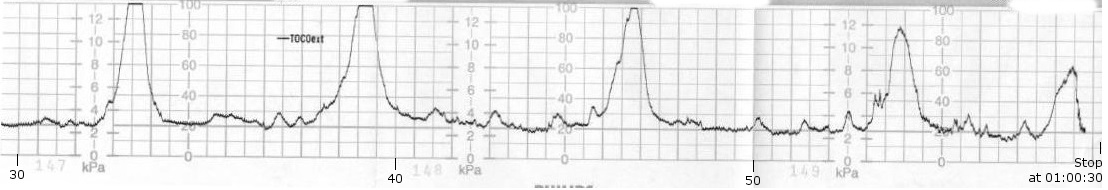
\includegraphics[scale=0.45]{imagens/toco.jpg} 		
 	\end{center}
 	%\legend{\cite{ref-islddatabase}}
 \end{figure}
 
 There are several disadvantages of Tocography. Important
 among them are:
 
 \begin{itemize}[leftmargin=*,labelsep=5.8mm]
 	\item	Inter and intra-personal variation in interpretation of CTG
 	trace \cite{ref-bernardes}.
 	\item	Sometimes there is shift (either up or down) in baseline of
 	signal which makes interpretation difficult. This is known as
 	baseline wandering \cite{ref-marques}. 	
 \end{itemize}
 
 This paper focuses on using fuzzy classification techniques, using Electrohysterogram (EHG) signals, to detect the onset of labor. As there is no current
 published information concerning fuzzy classification of EHG recordings, we propose to investigate, in this study, the potentialities of this method to determine a possible separation between effective
 contractions and non-effective contractions without the CTG disavantages.
 



%Please use the command \citep{ref-journal} for the following MDPI journals, which use author-date citation: Arts, Econometrics, Economies, Genealogy, Humanities, IJFS, JRFM, Laws, Religions, Risks, Social Sciences.


%%%%%%%%%%%%%%%%%%%%%%%%%%%%%%%%%%%%%%%%%%
\section{Materials}

\subsection{The Icelandic 16-electrode	Electrohysterogram Database}



A base de dados utilizada neste trabalho foi obtida entre 2008 e 2010 nos hospitais Landspitali University Hospital, Akureyri
Hospital e Akureyri Primary Health Care Centre na Islândia. Foram feitas 122 medidas (recordings) em 45 mulheres grávidas, onde 32 foram analisadas repetidamente durante o período de gravidez, participando de duas a sete vezes. As sessões ocorreram no terceiro trimestre da gestação (112 gravações) e durante o trabalho de parto(labor) (10 gravações).  Esta base inclui dados de tocodinamometria, anotações de eventos e informações obstétricas das participantes. Todos os dados foram obtidos com o consentimento dos participantes e os protocolos foram aprovados pelo Comitê Nacional de Bioética da Islândia (VSN 02-006-V4) \cite{ref-islddatabase}.

Um {\em grid} de $4x4$ eletrodos monopolares reutilizáveis de Ag/AgCl foi disposto no abdômen das pacientes conforme pode ser visto na Figura \ref{abd_elec} 


 \begin{figure}[H]
 	\caption{\label{abd_elec} Posição ideal do {\em grid} de 16 eletrodos. Os eletrodos pretos representam o {\em ground} do paciente.}
 	\begin{center}
 		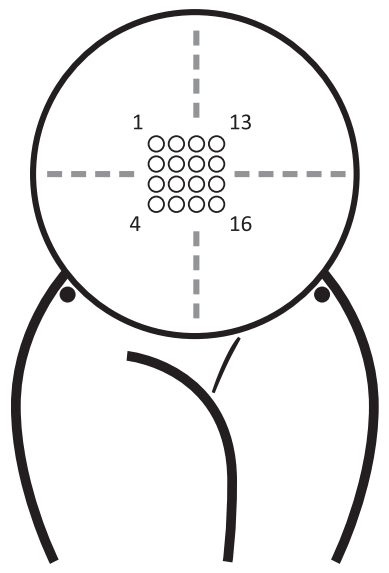
\includegraphics[scale=0.40]{imagens/abd_elec.png} 		
 	\end{center}
 	%\legend{\cite{ref-islddatabase}}
 \end{figure}

As medidas foram realizadas utilizando um equipamento de aquisição de dados fisiológicos de 16 canais (Embla A10). Um filtro {\em anti-aliasing} com corte em 100Hz foi usado, porém nenhum filtro passa-alta foi implementado. A taxa de amostragem do sinal foi de 200Hz, com uma resolução de 16 bits.  \cite{ref-islddatabase}.



 

%%%%%%%%%%%%%%%%%%%%%%%%%%%%%%%%%%%%%%%%%%
\section{Materials and Methods}

Materials and Methods should be described with sufficient details to allow others to replicate and build on published results. Please note that publication of your manuscript implicates that you must make all materials, data, computer code, and protocols associated with the publication available to readers. Please disclose at the submission stage any restrictions on the availability of materials or information. New methods and protocols should be described in detail while well-established methods can be briefly described and appropriately cited.

Research manuscripts reporting large datasets that are deposited in a publicly available database should specify where the data have been deposited and provide the relevant accession numbers. If the accession numbers have not yet been obtained at the time of submission, please state that they will be provided during review. They must be provided prior to publication.

Interventionary studies involving animals or humans, and other studies require ethical approval must list the authority that provided approval and the corresponding ethical approval code. 
 
 
%%%%%%%%%%%%%%%%%%%%%%%%%%%%%%%%%%%%%%%%%%
\section{Results}

This section may be divided by subheadings. It should provide a concise and precise description of the experimental results, their interpretation as well as the experimental conclusions that can be drawn.


%%%%%%%%%%%%%%%%%%%%%%%%%%%%%%%%%%%%%%%%%%
\subsection{Subsection}

\subsubsection{Subsubsection}

Bulleted lists look like this:
\begin{itemize}[leftmargin=*,labelsep=5.8mm]
\item	First bullet
\item	Second bullet
\item	Third bullet
\end{itemize}

Numbered lists can be added as follows:
\begin{enumerate}[leftmargin=*,labelsep=4.9mm]
\item	First item 
\item	Second item
\item	Third item
\end{enumerate}

The text continues here.

\subsection{Figures, Tables and Schemes}

All figures and tables should be cited in the main text as Figure 1, Table 1, etc.

 \begin{figure}[H]
 	\caption{\label{beer}This is a figure, Schemes follow the same formatting. If there are multiple panels, they should be listed as: (\textbf{a}) Description of what is contained in the first panel. (\textbf{b}) Description of what is contained in the second panel. Figures should be placed in the main text near to the first time they are cited. A caption on a single line should be centered.}
 	\begin{center}
 		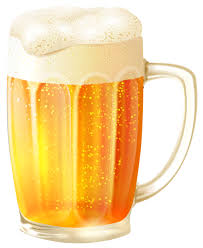
\includegraphics[scale=0.40]{imagens/beer.jpg} 		
 	\end{center}
 	%\legend{\cite[]{pll analog}}
 \end{figure}  



\begin{table}[H]
\caption{This is a table caption. Tables should be placed in the main text near to the first time they are cited.}
\centering
%% \tablesize{} %% You can specify the fontsize here, e.g.  \tablesize{\footnotesize}. If commented out \small will be used.
\begin{tabular}{ccc}
\toprule
\textbf{Title 1}	& \textbf{Title 2}	& \textbf{Title 3}\\
\midrule
entry 1		& data			& data\\
entry 2		& data			& data\\
\bottomrule
\end{tabular}
\end{table}

\subsection{Formatting of Mathematical Components}

This is an example of an equation:

\begin{equation}
\mathbb{S}
\end{equation}

%% If the documentclass option "submit" is chosen, please insert a blank line before and after any math environment (equation and eqnarray environments). This ensures correct linenumbering. The blank line should be removed when the documentclass option is changed to "accept" because the text following an equation should not be a new paragraph. 
Please punctuate equations as regular text. Theorem-type environments (including propositions, lemmas, corollaries etc.) can be formatted as follows:
%% Example of a theorem:
\begin{Theorem}
Example text of a theorem.
\end{Theorem}

The text continues here. Proofs must be formatted as follows:

%% Example of a proof:
\begin{proof}[Proof of Theorem 1]
Text of the proof. Note that the phrase `of Theorem 1' is optional if it is clear which theorem is being referred to.
\end{proof}
The text continues here.


%%%%%%%%%%%%%%%%%%%%%%%%%%%%%%%%%%%%%%%%%%
\section{Discussion}

Authors should discuss the results and how they can be interpreted in perspective of previous studies and of the working hypotheses. The findings and their implications should be discussed in the broadest context possible. Future research directions may also be highlighted.


%%%%%%%%%%%%%%%%%%%%%%%%%%%%%%%%%%%%%%%%%%
\section{Conclusions}

This section is not mandatory, but can be added to the manuscript if the discussion is unusually long or complex.

%%%%%%%%%%%%%%%%%%%%%%%%%%%%%%%%%%%%%%%%%%
\vspace{6pt} 





%%%%%%%%%%%%%%%%%%%%%%%%%%%%%%%%%%%%%%%%%%
\conflictsofinterest{The authors declare no conflict of interest.} 


%=====================================
% References, variant A: internal bibliography
%=====================================
\begin{thebibliography}{999}
	
%% Reference 1
\bibitem[T.L. Weissgerber, L.A. Wolfe (2006)]{ref-weisswolfe}
T.L. Weissgerber, L.A. Wolfe. Physiological adaptation in early human pregnancy: adaptation to balance maternal-fetal demands. {\em Appl. Physiol. Nutr. Metab.} {\bf 2006}, {\em 31}, 1-11.

%% Reference 2
\bibitem[N. Hatfield (2013)]{ref-hatfield}
N. Hatfield. References. In {\em Introductory maternity and paediatric nursing}, 3rd ed.; Wolters Kluwer Health: Albuquerque, USA, {\bf 2013}; ISBN: 9781451147025.		

%% Reference 3
\bibitem[J. Bernardes, A. Costa-Pereira, D. Ayres-de-Campos, H. Van Geijn, and L. Pereira-Leite. (1997)]{ref-bernardes}
J. Bernardes, A. Costa-Pereira, D. Ayres-de-Campos, H. Van Geijn, and L. Pereira-Leite. Evaluation of interobserver agreement of Cardiotocograms {\em International Journal of Gynaecology \& Obstetrics.} {\bf 1997}, {\em 57}, 33-37.

%% Reference 4
\bibitem[J. A. Marques, P. C. Cortez, J. P. Madeiro, and F. S. Schlindwein (2013)]{ref-marques}
J. A. Marques, P. C. Cortez, J. P. Madeiro, and F. S. Schlindwein. Computerized Cardiotocography analysis system based on Hilbert Transform {\em Expert System with Applications.} {\bf 2013}, {\em 40}, 7159-7658.		
	
%% Reference 5
\bibitem[Alexandersson, A. { \em et al} (2015)]{ref-islddatabase}
Alexandersson, A. { \em et al}.  The Icelandic 16-electrode electrohysterogram database. {\em Sci. Data 2:150017} {\bf 2015}, doi: 10.1038/sdata.2015.17.


	




%% Reference expl
%\bibitem[Author (year)]{ref-journal}
%Lastname, F.; Author, T. The title of the cited article. {\em Journal Abbreviation} {\bf 2008}, {\em %10}, 142-149.

%% Reference 2
%\bibitem[Author (year)]{ref-book}
%Lastname, F.F.; Author, T. The title of the cited contribution. In {\em The Book Title}; Editor, F., Meditor, A., Eds.; Publishing House: City, Country, 2007; pp. 32-58.
\end{thebibliography}

% The following MDPI journals use author-date citation: Arts, Econometrics, Economies, Genealogy, Humanities, IJFS, JRFM, Laws, Religions, Risks, Social Sciences. For those journals, please follow the formatting guidelines on http://www.mdpi.com/authors/references

%=====================================
% References, variant B: external bibliography
%=====================================
%\externalbibliography{yes}
%\bibliography{references}

%%%%%%%%%%%%%%%%%%%%%%%%%%%%%%%%%%%%%%%%%%
%% optional
%\sampleavailability{Samples of the compounds ...... are available from the authors.}

%%%%%%%%%%%%%%%%%%%%%%%%%%%%%%%%%%%%%%%%%%
\end{document}

